\chapter{Inference}
\label{ch:inference}
\begin{flushright}
\emph{A syllogism has 3 parts; therefore, this is not a syllogism.}
\end{flushright}
\minitoc

By inference we mean deduction and abduction;  induction is regarded a form of learning.

What are the computational bottlenecks?  How to speed things up?

\section{Some background}

\subsection{Resolution}
\label{sec:resolution}

In essence, the resolution rule is:\\
\hspace*{1cm} $P \vee Q $\\
\hspace*{1cm} $\neg P \vee R$\\
\hspace*{1cm} --------------\\
\hspace*{1cm} $Q \vee R$

Resolution is a popular deduction technique for binary logic;  we will not use it but it is helpful to know.

\subsection{Horn clauses and Prolog}
\label{sec:Prolog-Horn-intro}

In essence, a Horn clause is a rule of the form:\\
\hspace*{1cm} \begin{tabular}{l l}
(Prolog notation) &  \texttt{A :- B, C, D, ...}\\
(logic notation)  &  $A \leftarrow B, C, D, ...$
\end{tabular}

The Horn form makes deduction particularly efficient because it is like IF-THEN rules in production systems.  Resolution in Horn form is the basis of Prolog.

\subsection{Forward- and backward- chaining}

These are deduction algorithms.

Forward-chaining \textit{starts with the premises}, and applies deduction steps in the forward direction, to try to arrive at conclusion(s).  A goal (conclusion) may be specified as the search termination criterion;  if not, it is called goal-less forward-chaining.

Backward-chaining \textit{starts with the goal to be proven}, and applies deduction steps in the backward direction.  The search graph terminates with nodes that are the premises.

\subsection{Complexity of inference}

Some facts:

1.  Satisfiability in binary \textbf{first-order logic} is semi-decidable (ie, it terminates in finite time if a proof exists, but may never terminate if a proof does not exist)

2.  SAT for binary \textbf{propositional logic} is NP-complete.

3.  \textbf{Propositional Bayesian network} inference is \#P-complete (ie, it is as hard as returning the number of solutions to an NP-complete problem).

4.  The \textit{naive} algorithm for propositional Bayesian network inference is $O(n 2^n)$ where $n$ is the number of nodes.

5.  Pearl's message-passing algorithm is an \textit{exact} algorithm for propositional Bayesian network inference;  therefore it also requires non-polynomial time in the worst case.

6.  Pearl's algorithm, when operating on trees, is linear time.  But trees seem to be insufficient for AGI reasoning.

7.  SAT for the \textbf{propositional Horn} subclass of binary logic, can be performed in linear time.  My very simple algorithm for Bayesian inference is analogous to Horn deduction\footnote{The term Horn can only be used to describe binary logic:  a Horn clause is a clause with exactly one positive literal.  $\mathcal{PZ}$ logic has a Horn-like form, but the distinction between positive and negative literals disappears in logics with numerical truth values.}.  Prolog owes its efficiency to SLD resolution which is also Horn-based.

\section{Nonmonotonicity and redundancy}

\subsection{Handling exceptions (nonmonotonic reasoning)}
\label{sec:exceptions}

Fuzzy reasoning can sometimes lead to unsound conclusions, for example:\\
\textit{1. Mary has cybersex with many partners.\\
2. Cybersex is a kind of sex.\\
3. Therefore, Mary has many sex partners.\\
4. A person who has many sex partners has a high chance of STDs.\\
5. Therefore, Mary has a high chance of STDs.}

What's wrong with this example?  On the one hand, we should admit that cybersex is sex (it is a borderline case), but it lacks certain prominent features of sex, such as physical contact (which is not necessarily a \textit{defining} feature of sex).  Thus, if we carry on reasoning with the idea that cybersex is sex, we may get unsound conclusions.  The key to resolving this problem is to recognize ``cybersex is sex'' with \textbf{qualifications} such as ``but it is sex without physical contact''.

If we have a rule saying that ``sex transmits certain diseases'', we may have to attach the exception ``only if the sex involves physical contact''.  In the end, our rules may be inundated with possibly infinitely many exceptions.  How can we get out of this problem?

\citep*{Wang1994}, \citep*{Wang2006} provided a solution, which I essentially adopt.  His idea is not to store the exceptions to rules, but instead allow a \textit{multitude} of rules to fire, calculate the ``confidence'' (\S\ref{sec:confidence}) of each conclusion, and pick the conclusion with the highest confidence.  This allows us to handle exceptions relatively easily.

\section{Deduction}
\label{sec:deduction}

\subsection{Predicate logic and substitution management}
\label{sec:substitution-management}
\index{substitution!management}

We have argued that propositional (0th-order) logic is inadequate for AGI.  The situation is illustrated as follows:
\begin{figure}[H]
\centering
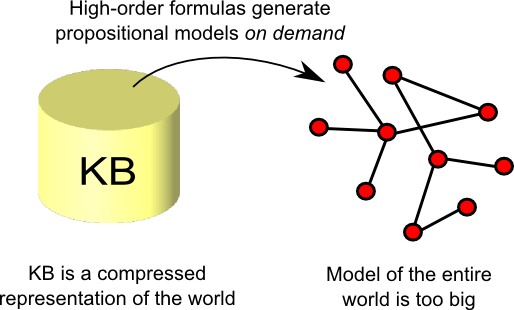
\includegraphics{KBMC-illustrated.png}
\end{figure}
This is known as KBMC (knowledge-based model construction).  What it means is that we need to \textbf{fetch} logical rules from the KB and \textbf{instantiate} those rules to form the propositional Bayesian networks upon which probabilities are propagated.
\index{KBMC (knowledge-based model construction)}

Substitution management in first-order logic provers is quite complicated.  This is famously explained in classics such as SICP \citep*{Abelson1984}, where the authors advocated using \textbf{lazy sequences}, also known as \textbf{streams}.

Think of a sequence of \textbf{solutions} attached to each variable node of the proof tree.  Each solution consists of a \textbf{substitution} and a \textbf{TV}.  When we carry out an operation between 2 variables, say $X^1 \varodot X^2$, we are not just dealing with 2 objects, but with 2 \textit{sequences} of possible solutions.  Let's denote the sequences as $X^1 = \{ x^1_1, x^1_2, ... \} $ and $X^2 = \{ x^2_1, x^2_2, ... \}$.  For each solution of each sequence, we need to:
\begin{compactenum}[1.]
\item  Match the 2 substitutions ($x^1_i.\mbox{sub}$ and $x^2_j.\mbox{sub}$), ie, see if they are compatible, and if so, merge the 2 substitutions.\\
       Let's denote the matching operation as $(x^1_i.\mbox{sub} \bowtie x^2_j.\mbox{sub})$.
\item  If the substitutions are compatible, perform the calculation of the CPT (conditional probability table).\\
       Let's denote this operation as $(x^1_i.\mbox{TV} \varodot x^2_j.\mbox{TV})$.
\end{compactenum}
Now denote the combined action of $\bowtie(\cdot, \cdot)$ and $\varodot(\cdot, \cdot)$ as $\heartsuit(x^1_i, x^2_j)$.  Then what we need to calculate can be expressed as:
\begin{equation}
X^0 = \heartsuit( X^1 \times X^2 \times ... \times X^n)
\end{equation}
where $\times$ is Cartesian product, and $\heartsuit$ is extended as an n-ary operation.  Note that each $X^i$ is a (lazy) sequence, so this formula is very succinct.  Further, we can ``curry'' the function $\heartsuit$ so that:
\begin{equation}
\heartsuit \cdot ( X^1 \times X^2 \times ... \times X^n) = (((\heartsuit \cdot X^1) \cdot X^2) \cdot ... )
\end{equation}
where we have made use of the associativity of $\varodot$ (see eqn \ref{eqn:P-and-or-associativity}).  The final RHS is what we will be coding.  It is quite amazing to realize that the proof tree in our program is actually many propositional Bayes nets overlaid together.

\subsection{Pure probabilistic inference}
\label{sec:P-inference}

%The $\mathcal{P}$ inference algorithm is similar to $\mathcal{Z}$ inference (Algorithm \ref{algorithm1}) except that probabilistic inference can be ``abductive'' --- a conditional probability can work in the reverse direction via Bayes theorem --- thus the branching factor of the search would be higher.
%
%\begin{algorithm}
%\caption{backward-chaining P inference}
%\label{algorithm2}
%\begin{algorithmic}[1]
%
%\REQUIRE a knowledgebase $KB$, a list of query goals $G$ \\
%\ENSURE $p =$ probability of $G$.
%
%\REPEAT
%	\STATE choose a literal $L$ from the list $G$, removing it from G
%	\STATE find a rule $X_0 \leftarrow \bigcurlyvee \bigcurlywedge X_{ij} $ such that\\
%			 $L$ unifies with one of the $X_{ij}$'s, including $X_0$\\
%	\COMMENT{ if $X_{ij}$ is null, $X_0$ is a fact in $KB$ }
%	\STATE add the $X$'s to the list $G$, except the one that unifies with $L$ \\
%	\STATE if depth of recursion $< h$ \\
%			 recurse to resolve the new list of goals $G$ \\
%\UNTIL{ there are no more applicable rules in $KB$. }
%
%\end{algorithmic}
%\end{algorithm}

Backward-chaining algorithms in binary logic are relatively familiar to us as they are explained in most AI textbooks.  One of the simplest backward-chaining algorithms is the SLDNF resolution\footnote{SLDNF stands for ``Linear Selection of Definite clauses, with Negation as Failure''.} used in Prolog (see \S\ref{sec:Prolog-Horn-intro}).  Originally I tried to adapt SLDNF resolution for probabilistic inference, but was doing a rather sloppy job of it.  Thanks to Abram Demski who pointed out that my ``Prolog trick'' could actually be replaced with exact Bayesian inference via a technique known as factor graphs, our inference algorithm is now on very good theoretical foundation.
\index{factor graphs}
\index{Bayesian networks!inference}
\index{Bayesian networks!factor graphs}
\index{SLDNF resolution}

TO-DO: There should be a mechanism to prune low-probability (or should it be low-confidence?) branches early on in the search.

%The solution to \#1 is to use 0.5 as the substitute for unknown probabilities.

%The solution to \#2 is to use only local dependencies.

%Case \#1:
%\begin{figure}[H]
%\centering
%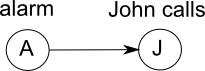
\includegraphics{BayesNet-alarm-John.png}
%\end{figure}
%\textbf{Forward inference}: the answer is simply what is given: $P(J|A)$\\
%\textbf{Backward inference (abduction)}: we seek $P(A|J)$ which is given by Bayes rule:\\
%$$ P(A|J) = \frac{P(J|A)P(A)}{P(J)} $$
%and we search for values of $P(A)$ and $P(J)$; If they don't exist we substitute with 0.5.

%It seems that we need to record the rule during inference.  When the subgoals are all found we can obtain the head.  Is there a way not to store the rules?  No.  Not only that, but we need to have backtrack ability too.

%Case \#2:
%\begin{figure}[H]
%\centering
%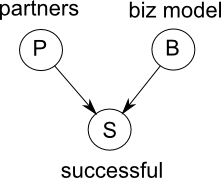
\includegraphics{BayesNet-successful-business.png}
%\end{figure}
%\textbf{Forward inference}: simply given by $P(S|P,B)$\\
%\textbf{Abduction}: given S, we can infer P and B.  "P or B" is a problem. How to represent that?  

\subsubsection{Factor graph algorithm}

Factor graphs are a way to unify probabilistic graphical models such as Bayesian networks and Markov networks.  The important thing to know is that factor graphs are isomorphic to the proof trees we construct during backward-chaining, and thus we can perform Bayesian belief propagation \textit{in situ} in the proof tree, very conveniently.  For example:
\begin{figure}[H]
\centering
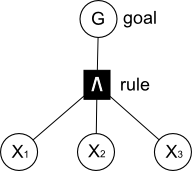
\includegraphics{simple-proof-tree.png}
\caption{Simple proof tree / factor graph}
\end{figure}
In this example we can see that the factor node (black square) is located exactly as the ``rule node'' in the proof tree, therefore we might as well label the node with its operator (``$\wedge$'').

\textbf{The algorithm:}  What we need to calculate, for a "goal" variable node $G$, is $P(G|K)$, where $K$ is the background knowledge.  $P(G)$ is called the prior distribution of $G$.

When the graph has no loops, then it is a tree, and the factor graph algorithm begins from the leaves of the tree to the root which is the goal node.  The leaves pass messages up to their parents, with each factor node performing a \textbf{sum-product} operation, until the messages reach the root.

Assume that we have a rule in the form:
\begin{equation}
H_1, H_2, ... \PimpL X_1 \varodot X_2 \varodot ...
\end{equation}
where the $H$'s stand for ``Heads''.  This is actually a compact way of stating more than 1 rule -- with each head corresponding to 1 rule\footnote{\{ To-do: explain why the multiple-head feature is desirable.\}}.  For simplicity's sake we assume number of $H$'s = 1.  For example:
\begin{figure}[H]
\centering
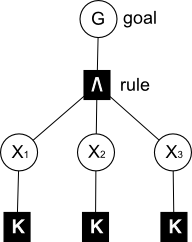
\includegraphics{simple-proof-tree2.png}
\caption{Simple factor graph in ``normal'' direction, with background knowledge}
\end{figure}

In the ``normal'' direction, our $G$ is $H$, so the calculation is pretty straightforward.  From now on we use the notational convention of omitting $P(\cdot)$ for probabilities; ie, $P(X)$ is written as $(X)$:
\begin{equation}
(G|K) = \sum_{X_i} (G|X_i)(X_i|K).
\end{equation}
The first factor on the RHS is the ``\textbf{factor}'' stored in the factor node.  The second factor is the \textbf{messages} coming from each $X_i$ node.  This is a simple sum-product operation.  The link to $K$ simply means that either the node's value is ``clamped'' or it is passing a message from further down the tree.

Next case, the direction is reversed:
\begin{figure}[H]
\centering
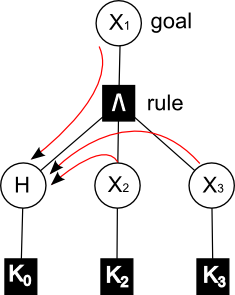
\includegraphics{simple-proof-tree3.png}
\caption{Simple factor graph in backward direction}
\end{figure}
Notice how the rule is not pointing to the goal $G$, and $G$ is now taking the place of $X_1$.  We need to apply Bayes rule twice:

First work out the 2-node case where $X_2, X_3, ...$ don't exist:\\
\begin{eqnarray*}
(G|K) &=& \frac{(K|G)(G)}{(K)} = \frac{(G)}{(K)} \sum_H (K|H)(H|G) \nonumber\\
      &=& (G) \sum_H \frac{(H|K)}{(H)} (H|G)
\end{eqnarray*}

General case:\\
\begin{eqnarray*}
(G|K) &=& \frac{(K|G)(G)}{(K)} = \frac{(G)}{(K)} \sum_H (K|H)(H|G) \nonumber\\
      &=& (G) \sum_H \frac{(H|K)}{(H)} \sum_{X_i} (H|G,X_1,X_2,...)(X_i|G) \nonumber\\
      &=& (G) \sum_H \frac{(H|K)}{(H)} \sum_{X_i} (H|G,X_1,X_2,...)(X_1)(X_2)...
\end{eqnarray*}

\subsubsection{Loopy inference}

\underconst

\subsection{Hybrid $\mathcal{B,P,Z}$ inference}

Rules, which are the building blocks of inference, can be of 4 types:

\begin{table}[H]
\parbox{3cm}{\caption{}}
\begin{tabular}{|l|l|} \hline
\multicolumn{2}{|c|}{\textbf{rules}}\\ \hline
mnemonic             & meaning\\ \hline
$\catB$              & Prolog statements of the form\\
                     & \qquad $L_0 \, \mbox{:--} \, L_1, L_2, L_3, ... $ \\
$\catZ$              & Fuzzy rules of the form\\
                     & \qquad $z_0 := \bigZandor \Gamma(z_{ij})$ \\
$\catPB$             & Bayesian network nodes specified by\\
                     & \qquad $X_0 \PimpL \bigPandor X_{ij};c_{ij}$ \\
$\catPZ$             & Specifications of $\catPZ$ distributions\\
                     & \qquad $X_0 := Beta(\mu,\sigma^2)$ \\
\hline
\end{tabular}
\end{table}

The type of a rule is determined by its ``head'' --- eg, if the head is a $\catB$ variable then the rule is a $\catB$ rule.  Using unified $\catPZ$ truth values, we can plug variables of any TV type into any rule.  So, the rule type only affects how the rule is interpreted, which will be explained below.

An example of a rule is:  ``almost Q'' means ``close to Q, but not being Q''.\\
The TV types of the predicates are:\\
\hspace*{1cm} ``almost Q'' --- $\catB$\\
\hspace*{1cm} ``close to Q'' --- $\catZ$\\
\hspace*{1cm} ``not Q'' --- $\catB$\\
So we can represent it with a $\catB$ rule:\\
\hspace*{1cm} $\mbox{almost } Q \leftarrow \mbox{ close-to } Q \wedge \neg Q$
Despite using a $\catB$ rule, the result of inference will be a $\catPZ$ truth value with binary character.  This is a good thing, because the idea of ``almost'' can be fuzzy in some cases, for example:\\
\hspace*{1cm} ``I heard that John almost got killed by the assassination?''\\
\hspace*{1cm} ``Not really, the bullet only hit his toe!''

To simplify things, I consider single inference steps.  A complete proof involves a series of such steps.

\subsubsection{$\catB$ rule:}

The $\catB$ rule can have 3 operators: $\wedge$, $\vee$, and $\neg$.  All we need to do is to show how to evaluate the operators for $\mathcal{P(Z)}$ values.  An example $\catB$ rule is:\\
\hspace*{1cm} \texttt{bachelor :- male $\wedge \; \neg$ married}

Case $\neg$ :  We need to convert the $\mathcal{P(Z)}$ distribution to one with a binary character.  This is done by setting the variance to a fixed value in the binary regime (\S\ref{sec:unifying-P(Z)}).  Then the result is negated by transforming the mean:
\begin{equation}
\mu ' = 1 - \mu
\label{eqn:1-minus-z-transform}
\end{equation}

Case $\wedge$ : Convert the $\mathcal{P(Z)}$ value to $\mathcal{P(B)}$ via eqn (\ref{eqn:mean-and-p}).  Then $P(A \wedge B) = P(A) P(B)$, assuming independence.

The variance is assigned a fixed value so that the resulting variable has binary character.  Note that the resulting variance is not affected by the variances of the premises because the aim of a $\mathcal{B}$ rule is to form a \textit{binary} judgment.

Case $\vee$ : Similar to above, with $P(A \vee B) = P(A) + P(B) - P(A)P(B)$, again assuming independence.

\subsubsection{$\catZ$ rule:}

$\catZ$ rules can have the operators $\Zand$ (= min), $\Zor$ (= max), $\Zneg$ ($= 1-z$) and the fuzzy modifier $\Gamma()$.  At this stage we ignore Soft min and max.  The $\Gamma()$'s are applied before the other operators.

Case $\Gamma$() : If $z_0 := \Gamma(z_1)$ and $z_1$ is given by the probability density function $f_1(z1)$, then the probability density of $z_0$ would be given by:
\begin{equation}
f_0(z_0) = f_1(\Gamma^{-1}(z_0)) \left | \frac{d\Gamma^{-1}}{dz_0} \right |
\end{equation}
which is explained in \citep*{Wikipedia2008}.  If $\Gamma()$ is the Gaussian function given in eqn (\ref{eqn:fuzzy-moderator-Gaussian}) then\\
$$ f_0(z_0) = f_1(\pm \sigma \sqrt{-2 \ln z_0} + z^*) \left | \frac{\sigma}{z_0 \sqrt{-2 \ln z_0}} \right | $$
but there is a glitch:  $\Gamma^{-1}()$ has 2 pieces, and their contributions must be summed up piecewise.  Sometimes the resulting distribution looks irregular, for example:
\begin{figure}[H]
\centering
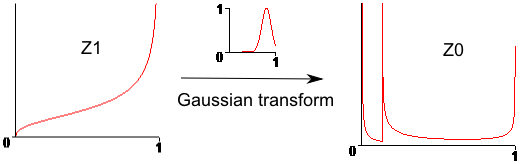
\includegraphics[scale=0.9]{Z1-Gaussian-transform-to-Z0-ugly.png}
\end{figure}
but we can approximate it with a Beta distribution by preserving the mean and variance.  The irregular appearance does not matter that much if we only care about the mean and variance.  I have obtained the approximation formula by numerical integration and nonlinear regression on randomly generated samples, as follows ($m_1$ = mean of input, $m_0$ = mean of result):
\begin{figure}[H]
\centering
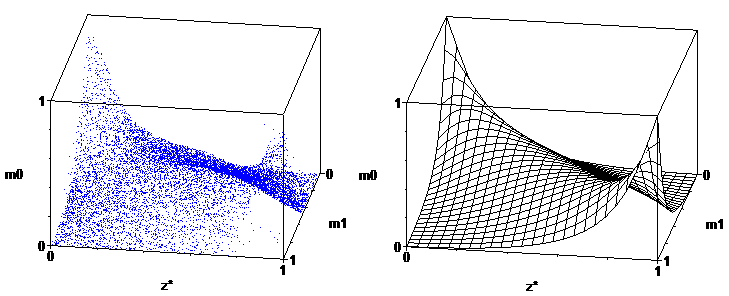
\includegraphics[scale=0.7]{Gaussian-fuzzy-modifier-regression-result.png}
\caption{Gaussian fuzzy modifier:  empirical data and result of regression}
\end{figure}

Case $\Zneg$ :  Simply negate the $\catPZ$ distribution by eqn (\ref{eqn:1-minus-z-transform}) with variance unchanged.

Case $\Zor$ :  Given $z_0 := z_1 \Zor z_2$, ie $z_0 = max(z_1, z_2)$.  What we need to do here is to calculate the PDF of a random variable given as a function of two other random variables.  The procedure is given in many textbooks.

Here $\catP$ denotes probability measure which is a set function, $F(t)$ denotes CDF's, $f(t)$ denotes PDF's.

%Define the region $D_0 := \{ (z_1,z_2): \widetilde{\wedge}(z_1,z_2) \leq z_0 \}$.
%\begin{eqnarray}
%F_0(z_0) & = & \mathbf{P}(Z_0 \leq z_0)\\
%         & = & \mathbf{P}((Z_1,Z_2) \in D_0)\\
%         & = & \iint_{D_0} f_{12}(z_1,z_2) dz_1 dz_2
%\end{eqnarray}
%If we assume $Z_1, Z_2$ independent then $f_{12}(z_1,z_2) = f_1(z_1) f_2(z_2)$.

\hspace*{1.2cm} $ F_0(t) = \mathbf{P}(Z_0 \leq t)$\\
\hspace*{2cm} $= \mathbf{P}(\Zor(Z_1,Z_2) \leq t)$\\
\hspace*{2cm} $= \mathbf{P}(max(Z_1,Z_2) \leq t)$\\
\hspace*{2cm} $= \mathbf{P}(Z_1 \leq t \wedge Z_2 \leq t)$\\
\hspace*{2cm} $= \mathbf{P}(Z_1 \leq t) \, \mathbf{P}(Z_2 \leq t)$ \quad assuming $Z_1, Z_2$ independent\\
\hspace*{2cm} $= F_1(t) F_2(t)$\\
where $$ F_1(t) = \int_0^t f_1(z_1) dz_1 , \quad F_2(t) = \int_0^t f_2(z_2) dz_2$$

%The result we want is: $ f_0(t) = dF_0(t) / dt $
The result we want is:
\[ f_0(t) = \frac{dF_0(t)}{dt} = F_2(t) \frac{dF_1(t)}{dt} + F_1(t) \frac{dF_2(t)}{dt} \]
and we need to apply Leibnitz's Rule.\footnote{For a function of t defined by: $$ F(t) := \int_a(t)^b(t) \Phi(x,t) dx $$ its differentiation is given by Leibnitz's Rule: $$ \frac{dF(t)}{dt} = \int_{a(t)}^{b(t)} \frac{\partial\Phi(x,t)}{\partial t} dx + \Phi(b(t),t) \frac{db(t)}{dt} - \Phi(a(t),t) \frac{da(t)}{dt} $$ }  Then we get:
\begin{equation}
f_0(t) = f_1(t) F_2(t) + f_2(t) F_1(t)
\end{equation}

%If it is $min()$:\\
%\hspace*{1.2cm} $ F_0(t) = \mathbf{P}(\widetilde{\vee}(Z_1,Z_2) \leq t)$\\
%\hspace*{2cm} $\approx \mathbf{P}(min(Z_1,Z_2) \leq t)$\\
%\hspace*{2cm} $= \mathbf{P}(Z_1 \leq t \vee Z_2 \leq t)$\\
%\hspace*{3cm} assuming $Z_1, Z_2$ independent:\\
%\hspace*{2cm} $= \mathbf{P}(Z_1 \leq t) + \mathbf{P}(Z_2 \leq t) - \mathbf{P}(Z_1 \leq t) \mathbf{P}(Z_2 \leq t)$\\
%\hspace*{2cm} $= F_1(t) + F_2(t) - F_1(t) F_2(t)$

This function $f_0$ has an interesting property:  it appears to add up the distributions $f_1$ and $f_2$, \textit{with the one on the right being dominant}, ie, giving the biggest contribution of probability mass (or area under the curve).  Some examples are as follows:
\begin{figure}[H]
\centering
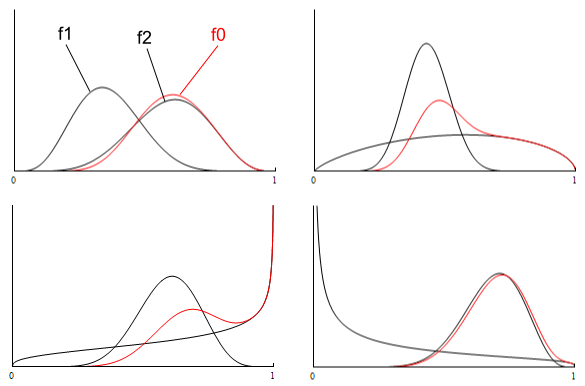
\includegraphics[scale=0.8]{A-ZOR-B-examples.png}
\caption{$z_0 := z_1 \, \Zor \, z_2$}
\end{figure}

%Some observations about the shapes:
%
%A. When the 2 inputs are unimodal:
%
%1. If they are narrow (ie small variance) and fairly separated, the mode on the right almost completely dominates; deviation is negligible.\\
%2. When the 2 modes are close, the mean of the result shifts to the right and variance decreases (the peak gets narrower).\\
%3. If any one input is broad (ie large variance), the result will shift to the right.  The change in variance is ambiguous.
%
%new mean = right mean + (amount of shift)
%amount of shift = f( how close they are, how broad they are)
%if close then new variance = narrower
%
%B. When 1 of the inputs has infinity on one side or both:
%
%1. If infinity is on both sides, the result will retain the infinity on the right, plus a small second peak near the second input (which is shifted slightly to the right).  It may be approximated by a J shape with a or b = 1 on one side.\\
%2. If infinity occurs on the right only (J shape), that infinity dominates the result, and the second input has a rather slight effect.\\
%3. If infinity occurs on the left, the second input will dominate.  Deviation from the second input is very slight.
%
%C. If both inputs have infinities:
%
%1. When 2 J shapes are crossed, the right side dominates, and there is a very slight shift to the left (but the stats seem to indicate that the shift can be big).  Sometimes, but rarely, to the right too -- why? Well the reason can be quite obscure.\\
%2. With a U shape and a J shape to the left, the result is a J shape to the right but with a small peak near the left end.  May be difficult to approximate (or use the power distribution?)\\
%3. With a U shape and a J shape to the right, the result is a J shape to the right with a greater variance (ie more polarized).  The degree of extra polarization depends on the contribution of the U shape (whether it's heavy on the right side).\\
%4. With 2 U shapes, the result is a J shape.

Once again, we approximate by preserving the mean and variance; The irregular appearance is not so important.  By looking at the following graph we can see that the mean of the result ($m_0$) is mostly dominated by $m_2$ which is the mean of the input further to the right (ie, $m_2 > m_1$).  There is sometimes a slight shift to the right relative to $m_2$ (the dots above the $x=y$ line), but it seems insignificant and may be ignored.  In other words, the fuzzy inference rule is very simple:  \textit{the mean of the result is just the greater mean of the 2 inputs}.  A similar graph shows that the variance of the result is also approximately equal to the variance of the rightmost input.
\begin{figure}[H]
\centering
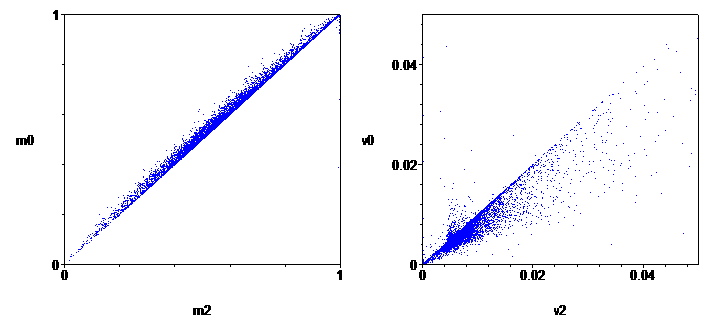
\includegraphics[scale=0.8]{z1-OR-z2-M-and-V-plots.png}
\caption{Plots of mean and variance; output vs input}
\end{figure}

Case $\Zand$ : The result for $z_0 := z_1 \, \Zand \, z_2$ is similar (again assuming $Z_1, Z_2$ independent):
\begin{equation}
f_0(t) = f_1(t) + f_2(t) - f_1(t) F_2(t) + f_2(t) F_1(t)
\end{equation}

In summary, the fuzzy inference rules are:

\fbox{ \parbox{8cm}{
1. For $z_0 := \neg z_1$\\
\hspace*{0.3cm}  $\mu_0 = 1 - \mu_1$\\
\hspace*{0.3cm}  $v_0 = v_1$ \\
2. For $z_0 := z_1 \vee z_2$\\
\hspace*{0.3cm} $\mu_0 = max(\mu_1, \mu_2)$\\
\hspace*{0.3cm} $v_0 = \left\{ \begin{array} {r@{\quad:\quad}l}
					v_1 & \mu_1 > \mu_2\\
					v_2 & \mu_2 > \mu_1 \end{array} \right.$\\
3. For $z_0 := z_1 \wedge z_2$\\
\hspace*{0.3cm} $\mu_0 = min(\mu_1, \mu_2)$\\
\hspace*{0.3cm} $v_0 = \left\{ \begin{array} {r@{\quad:\quad}l}
					v_1 & \mu_1 < \mu_2\\
					v_2 & \mu_2 < \mu_1 \end{array} \right.$\\
4. For $z_0 := \Gamma(z_1)$,
$$ \mu_0 = \frac{k_1+k_2}{\sigma_1} e^{- (m_1-z^*)^2 / \sigma_1^2 } $$
$$ v_0 = \frac{k_3}{\sigma_2} e^{- (z^* - \sqrt{3} m_1 + k_4)^2 / \sigma_2^2 } $$
\hspace*{0.3cm} where $\sigma_1 = k_1 (m_1+z^*-1)^2 + k_2 $ \\
\hspace*{1.4cm}     $\sigma_2 = k_5 (z^* + \sqrt{3} m_1 - k_6)^2 + k_7 $ \\
\hspace*{0.3cm} the $k$'s are regression parameters
}}

\subsubsection{$\catPB$ rule:}

A $\mathcal{P(B)}$ rule is of the form:\\
\hspace*{1cm} $X_0 := \bigPor \bigPand X_{ij};c_{ij}$

To simplify things, we do not implement the Bayesian network algorithm, instead we only perform the calculation $X_0$ from $X_{ij}$ in one direction.  This is an extreme simplification of probability logic, but it may already be sufficient for common-sense reasoning.  We will try this first and see how far it can go.

The $\catPZ$ variables can be converted to $\catPB$ variables via eqn (\ref{eqn:mean-and-p}).  Then the $\catPB$ value of the consequent can be obtained via straightforward application of probabilities, eg:\\
%\hspace*{1cm} $P(X_1 \wedge X_2) = \sum_{i=1,2} P(X_1 \wedge X_2 \; | \; P(X_i)) \; P(X_i)$ \\
\hspace*{1cm} $ P(X_1 \wedge X_2) = (1-p_1)(1-p_2)(1-c_1)(1-c_2) \; + $ \\
\hspace*{3.5cm} $ (1-p_1)p_2(1-c_1)c_2 \; + $ \\
\hspace*{3.5cm} $ p_1(1-p_2)c_1(1-c_2) \; + $ \\
\hspace*{3.5cm} $ p_1 p_2 c_1 c_2 $ \\
where $p_i = P(X_i)$.  Note that it reduces to the binary case when $c_1 = c_2 = 1$.  The result is then converted back as a $\mathcal{P(Z)}$ distribution (with binary character).

\subsubsection{$\catPZ$ rule:}

We do not use truly $\catPZ$ rules because they are too complex and not needed for common-sense reasoning.  The $\catPZ$ rules we have are simpler operations that allow us to manipulate the $\catPZ$ distributions of variables.

We can directly assign the mean and variance to a $\catPZ$ variable:\\
\hspace*{1cm} $X_0 := Beta(z; a, b)$

Or we can fix the probability at a particular point $z*$'s neighborhood.  For example, ``the probability of Mary being 0.9 fat is 0.1''.

%\textcolor{red}{The stuff below this line are just my notes and may contain many errors.}
%\hrulefill

%In the probabilistic setting... we have to deal with adding rules and using the ``combination rule''... 
%
%\hspace*{1cm} \[ f = \frac{f_1 w_1 + f_2 w_2}{w_1 + w_2} \]

%The assumption is...?
%
%The confidence of the result is given by:\\
%\hspace*{1cm} \[ c = C(c_1, c_2) ? \]

%\subsection{Hybrid rules}
%\label{sec:hybrid-rules}
%
%Some rules may involve factors of various truth-value types.  For example, ``almost'' means ``close to, but not being'', which translates to this rule:\\
%\hspace*{1cm} $\mbox{almost } Q \leftarrow \mbox{ close-to } Q \wedge \neg Q$\\
%where the first factor is $\mathcal{Z}$, the second factor is $\mathcal{B}$.
%
%Maybe we should disallow $\mathcal{P}(\mathcal{Z})$-rules in the AGI because they are too sophisticated?
%
%The hybrid rules can be:\\
%\hspace*{1cm} \begin{tabular}{|l|l|l|l|l|} \hline
%                           & $\mathcal{B}$           & $\mathcal{Z}$                     & $\mathcal{P}(\mathcal{B})$ & $\mathcal{P}(\mathcal{Z})$\\ \hline
%                           & $\vee \wedge$           &                                   &            & \\
%$\mathcal{Z}$              & case H1                 & $\widetilde\vee \widetilde\wedge$ &                         & \\
%$\mathcal{P}(\mathcal{B})$ & $\curlyvee \curlywedge$ & case H2                           & $\curlyvee \curlywedge$ & \\
%$\mathcal{P}(\mathcal{Z})$ & case H3                 & case 8                            & case H4                 & $\widetilde\curlyvee \widetilde\curlywedge$ \\ \hline
%\end{tabular}
%
%TO-DO:  unfinished.

%\subsection{Unified $\mathcal{P(Z)}$ rules?}
%\label{sec:unified-BPZ-inference}
%
%This section is optional.  As far as inference goes, the rest of this chapter has outlined the algorithms.  Here we try to see how $\mathcal{B}$, $\mathcal{P}$, and $\mathcal{Z}$ can be unified under the most general logic, $\mathcal{P}(\mathcal{Z})$.  Such a logic may be desirable in machine learning, where the general form of $\mathcal{P}(\mathcal{Z})$-rules may allow us to perform the searching in a continuous space, and some of the rules will degenerate nicely into $\mathcal{B}$, $\mathcal{Z}$, and $\mathcal{P}(\mathcal{B})$ rules.  Anyway, it turns out that $\mathcal{P}(\mathcal{Z})$-rules are not that simple and degeneration is also complex.
%
%First, let's start with a general form of $\mathcal{Z}$-rule which is a function $\mathcal{Z} \times \mathcal{Z} \cdots \rightarrow \mathcal{Z}$:\\
%$$ z_0 := \widetilde{\bigvee_i}\, \widetilde{\bigwedge_j}\, \Gamma_{ij}(z_{ij}) $$
%where $\Gamma_{ij}$ are Gaussian functions with means $z^*_{ij}$ and variances $v_{ij}$ (in other sections we don't use the variance).  The interpretation of $\Gamma$ is:  $z^*_{ij}$ represent the optimal values, which results in $\Gamma = 1$, and when $z_{ij}$ deviates from $z^*_{ij}$, $\Gamma$ drops from 1.
%
%Now generalize this to the $\mathcal{P}(\mathcal{Z})$-rule which is a function $\mathcal{P}(\mathcal{Z}) \times \mathcal{P}(\mathcal{Z}) \cdots \rightarrow \mathcal{P}(\mathcal{Z})$.  Let's denote $\mathcal{P}(\mathcal{Z})$ variables as $\mathbf{W}$.  Each $\mathbf{W}$ is a Beta distribution with mean $z^*$ and variance $v$.  A $\mathcal{P}(\mathcal{Z})$-rule has the general form:\\
%\begin{equation}
%\mathbf{W}_0 \leftarrow \widetilde{\bigcurlyvee_i} \, \widetilde{\bigcurlywedge_j}\, \Gamma_{ij}(\mathbf{W}_{ij})
%\end{equation}
%which contains the parameters $z^*_{ij}$, $v_{ij}$, and $c_{ij}$ (from the probabilistic $\curlyvee \curlywedge$, \S\ref{sec:probabilistic-AND-OR}).  $\widetilde{\curlyvee} \widetilde{\curlywedge}$ is different from $\widetilde{\vee} \widetilde{\wedge}$ and $\curlyvee \curlywedge$, and the rule is interpreted as follows:
%
%\textbullet \, If the rule is $ \mathbf{W}_0 \leftarrow \Gamma_1(\mathbf{W}_1) $ we simply apply $\Gamma_1$ to the distribution $\mathbf{W}_1$.  The variance of $\mathbf{W}$ may change because of $\Gamma$.  This is covered in \hyperref[case8]{Case \#8}.
%
%\textbullet \, Suppose the rule is $ \mathbf{W}_0 \leftarrow \mathbf{W}_1 \, \widetilde{\curlyvee} \, \mathbf{W}_2 $.  In \hyperref[case8]{Case \#8} we considered how to plug a $\mathcal{P}(\mathcal{Z})$-variable into a $\mathcal{Z}$-rule.  There, the $\mathcal{Z}$-rule did not actively affect the probability distributions.  Now the $\widetilde{\curlyvee}$ adds a constraint on the probability of $\mathbf{W}_0$ based on the values $c_1, c_2$ (from eqn (\ref{eqn:probabilistic-AND-OR})).  So we add the constraint:\\
%\hspace*{1cm} $ P(z_0 = z^*_0 \, | \, z_1 = z^*_1, z_2 = z^*_2) = c_1 + c_2 - c_1 c_2 $\\
%where the RHS comes from eqn (\ref{eqn:probabilistic-AND-OR}).  The effect of this is to change the shape of $\mathbf{W}_0$ to ``sharper'' or ``broader''.  The sharper the shape, and thus the smaller the variance, the more certain we are that $z_0 = z^*_0$.  But the formula is incorrect because continuous probabilities at a point is meaningless.  So we need to say\\
%\hspace*{1cm} $ P(z_0 \in N(z^*_0) \, | \, z_1 \in N(z^*_1), z_2 \in N(z^*_2)) = c_1 + c_2 - c_1 c_2 $\\
%where N is the interval $[0,\frac{1}{2}]$ or $[\frac{1}{2},1]$, whichever $z$ is in, thus transforming $z$ as binary.
%
%\textbf{Degeneration of rules.}
%
%\textbullet \, A $\mathcal{P}(\mathcal{B})$-rule reduces to a $\mathcal{B}$-rule when $c_{ij} \rightarrow 1$ (\S\ref{sec:probabilistic-AND-OR}).\\
%\textbullet \, A $\mathcal{P}(\mathcal{Z})$-rule reduces to a $\mathcal{Z}$-rule when $c_{ij} \rightarrow 1$.\\
%\textbullet \, A $\mathcal{Z}$-rule reduces to a $\mathcal{B}$-rule when $\Gamma_{ij} \rightarrow I$, the identity function.\\
%\textbullet \, A $\mathcal{P}(\mathcal{Z})$-rule reduces to a $\mathcal{P}(\mathcal{B})$-rule when $\Gamma_{ij} \rightarrow I$.
%
%One problem is that when we say a $\mathcal{P}$-rule degenerates into a $\mathcal{B}$-rule, it can remain to be a $\mathcal{Z}$-rule with $\Gamma_{ij} = I$.  The rule itself cannot tell us which type it is.

\subsection{Inference of confidence}
\label{sec:confidenceInference}

Confidence was introduced in \S\ref{sec:confidence}.  There, I explained that:\\
1. The confidence of rules can be measured in a frequentist way\footnote{Note, however, that the confidence c is not a frequency; it is just related to the frequency. }\\
2. The confidence of ground facts must be inferred

The problem is, we must initially know the confidence of at least \textit{some} ground facts in order to infer those of others.  To this end, I propose a convention to assign all \textbf{raw sensory events} (eg, ``a camera's pixel records the RGB color \#556677 at time 012345'')  to have confidence 1 (and thus $\infty$ support).  (It should not have 0 confidence because that would mean, informally, that the statement is so weak as to have no support at all).

In general, each inference step involves a rule of the form:\\
\hspace*{1cm} A $\longleftarrow$ B, C, D, ...\\
where the rule has a frequentist confidence $c_R$, and the antecedents B, C, D,... each has an inferred confidence.  So how to calculate $c_A$ from $c_B, c_C, c_D,$ ...?

Let's start from the simplest case.  Consider the rule:\\
\hspace*{1cm} A $\leftarrow$\textemdash\textemdash\textemdash\textemdash\textemdash $\,$ B\\
\hspace*{1cm} ? \hspace*{0.8cm} $c_R$ \hspace*{0.7cm} $c_1$ \\
where \hspace*{0.4cm} $c_R$ = confidence of the rule\\
\hspace*{1.6cm} $c_1$ = confidence of the antecedent B\\
and we seek the formula for $c_0 := f(c_1, c_R)$.

By considering the following ``boundary'' cases:\\
(the numbers are confidences)\\
\hspace*{1cm} A $\leftarrow$\textemdash\textemdash\textemdash\textemdash\textemdash $\,$ B\\
\hspace*{1cm} (0) \hspace*{0.8cm} 0 \hspace*{0.8cm} 1\\
\hspace*{1cm} A $\leftarrow$\textemdash\textemdash\textemdash\textemdash\textemdash $\,$ B\\
\hspace*{1cm} (0) \hspace*{0.8cm} 1 \hspace*{0.8cm} 0 \\
\hspace*{1cm} A $\leftarrow$\textemdash\textemdash\textemdash\textemdash\textemdash $\,$ B\\
\hspace*{1cm} (0) \hspace*{0.8cm} 0 \hspace*{0.8cm} 0 \\
\hspace*{1cm} A $\leftarrow$\textemdash\textemdash\textemdash\textemdash\textemdash $\,$ B\\
\hspace*{1cm} (1) \hspace*{0.8cm} 1 \hspace*{0.8cm} 1\\
we surmise that $f(\cdot,\cdot)$ degenerates into binary AND.  In other words, we're seeking an operator that generalizes binary AND.  Naturally, this can be either probabilistic AND (the product rule) or fuzzy AND (min rule).

The min rule epitomizes the proverb ``a chain is only as strong as its weakest link''.  Its special property is that a rule of $< 1$ confidence can be repeatedly applied without decreasing the conclusion's confidence.

The probabilistic rule forces confidence to \textit{decay} in long inference chains, if the confidence of each step is $< 1$.

At this point it is hard to say which method is superior.

To recap:  Every rule has a frequentist confidence;  a ground fact's confidence is inherited from the rules that entail it.

Confidence is useful in 2 ways:
\begin{compactenum}[1.]
\item  As a termination criterion for proof-search:  A statement of low probability can still be significant, eg: ``it is highly unlikely that an AGI can be run on an APPLE $][$''.  A statement is insignificant if its confidence is close to 0.
\item  In belief revision, when 2 inference chains arrive at different conclusions, their confidences will decide which has the greater weight.
\end{compactenum}

\subsection{Putting it all together: the deduction algorithm}

We are now able to work out the deduction algorithm.  This algorithm can be very fast because:\\
1.  the logic is truth-functional, ie, it ignores long-range probabilistic dependencies\\
2.  the logic is algebraic, ie, it does not use the binary implication operator $\rightarrow$

Every rule in the logic is of the \textit{conditional form}:\\
\hspace*{1cm} A $\leftarrow$ $op$(B, C, D, ...)\\
where $op$ is one of the operators described earlier.

The deduction algorithm will be given a query goal, G.  It then seeks rules in the KB with G as the head:\\
\hspace*{1cm} G $\leftarrow$ $op$(X1, X2, X3, ...)\\
and it basically performs recursion with X1, X2, X3, ... as subgoals.

\begin{algorithm}[H]
\caption{simple backward chaining}
\alginout{a knowledgebase $KB$, a query $G$}
{the truth value of $G$}
\begin{algtab}
\alglabel{alg:simple-backward-chaining}

\algrepeatforever
get a list of rules potentially applicable to $G$\\

\addtocounter{algline}{-1}\algnonumber (we maintain an index of predicates so we can quickly find the rules with the same head predicate as $G$)\\

select an applicable rule $R$ whose head unifies with $G$\\
% \algand is not in the taboo memory\\

\algif{recursion has gone too deep \algor the (incomplete) proof is already too long}
\algreturn `fail'\\
\algend

evaluate the rule $R$\\
\addtocounter{algline}{-1}\algnonumber (recurse to evaluate the variables in the rule body)\\

\end{algtab}
\end{algorithm}
\vspace{-0.6cm}

The search space of this algorithm is a so-called \textbf{AND-OR graph} (or tree) that often appears in logic-based AI search.  Each AND is represented by a horizontal line (whose elements are the arguments of an operator and \textit{all} of them must be evaluated);  each OR is represented by a set of child branches (shown in red in the diagram) (whose elements are rules from the KB and only one needs to be selected).  Thus the search is basically a matter of selecting which rules to apply.
\begin{figure}[H]
\centering
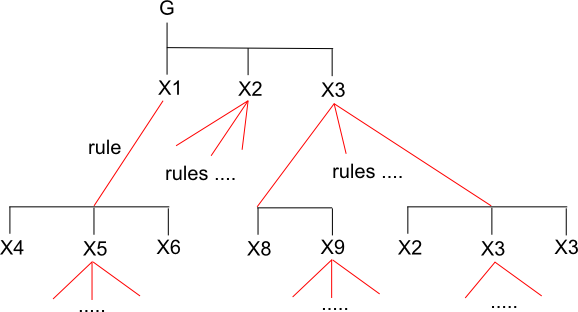
\includegraphics[scale=0.8]{and-or-graph.png}
% \caption{Plots of mean and variance; output vs input}
\end{figure}

\textbf{Complexity.}  If $m$ is the average number of rules applicable to a head predicate, $n$ is the average number of arguments for each rule, and $h$ is the depth of the search tree, then the size of the tree is $O((m \cdot n)^h)$.  Let me make a wild guess that $m \approx 30, n \approx 5, h \approx 5$, then size $\approx 10^{11}$.  This sounds manageable, but don't forget that the complexity of learning is the exponentiation of this!  So it is important to keep things simple at this stage.

\textbf{Efficient deduction.}\\
1.  Inference is often grounded by facts in \textbf{Working Memory} (ie, things that the AGI is currently paying attention to), though it may also be grounded by facts recalled from LTM (Long Term Memory).  Perhaps an efficient search algorithm should \textit{simultaneously} use backward chaining from the goal and forward chaining from ground facts under current attention.\\
2.  Given a head predicate, the KB server can quickly retrieve a list of all rules with that predicate by looking up an index.  Also, this list can be assumed to be sorted in order of confidence (remember that each rule is associated with a frequentist confidence).  This order may provide a basis for best-first / heuristic search\\
2.  Maybe the search should be randomized, and maybe it can start from the ``middle'' (ie, we generate an initial proof that is incorrect or incomplete, then repeatedly mutate it to make it correct)\footnote{This idea is inspired by the GSAT and WalkSAT algorithms for propositional logic.}.  This suggests using an evolutionary algorithm, but EA's may be slow. \{ TO-DO:  explore this idea further \}

Solving this search problem is very important because inductive learning also depends on such a search.

\section{Abduction}
\label{sec:abduction}

(Logic-based) abduction and induction are closely related;  they are 2 faces of the same coin.  In both cases we seek a hypothesis $H$ that together with background knowledge $B$, entails a positive example $e^+$:
$$ B \cup H \vdash e^+ $$
the only difference is that for abduction, $H$ is ground (ie, contains no variables); and for induction, $H$ is non-ground.

In classical logic, the algorithm for abduction is identical to deduction (backward chaining) except that the termination criterion is different.  In deduction the leaves of the search tree should be ground facts in the KB (which are believed to be true).  For abduction, the leaves should be so-called \textbf{abducibles}, which are propositions that can be assumed to be true.  For example, ``rain'' is a common occurrence and thus can be assumed to be true in order to account for the grass being wet.

Under probabilistic logic, we no longer need the notion of abducibles.  Interestingly, in this case the algorithm for abduction becomes almost identical to that of deduction, with the exception that deduction starts with an unknown fact whose truth is to be determined; whereas abduction starts with a known fact in need of explanations.  The 2 search spaces are exactly the same.

%Z abduction sometimes gives out-of-bounds Z values.\\
%\hspace*{1cm} $ z_1 \widetilde \vee z_2 = high $\\
%\hspace*{1cm} $ z_1 = low $\\
%\hspace*{1cm} $ \Rightarrow z_2 > 1.0 $
%
%Also, there are always 2 solutions, and they are within-bounds in the $z_1 > 0.5$ regime. Why?
%
%In fact, abduction using a rule with a point-Z-value is very unnatural.  Perhaps if we use $P(Z)$ the problem will be resolved?  But the ``2 roots'' problem seems to remain...
